\chapter{Introduction}
\section{Background and research purpose}
In the foreseeable future, electrification of ocean systems, renewable ocean power sources, and ocean energy networks will be necessary because they can help to accelerate the growth of ocean renewable energy and explore the mystery of the ocean \cite{Orekan, Randhawa2015}. 
To achieve electrification in the ocean, it is necessary to deploy corresponding sensor networks, which can reliably operate in underwater environment, %and process the data received by underwater sensors 
to monitor as well as control the electrification system in a timely manner (Figure \ref{fig:underwater sensor networks}). 
In addition, underwater sensors are also essential equipments for studying the marine environment \cite{Heidemann2012, Wu2020}. 
They can easily and flexibly explore underwater terrain and ecological environment, which provides convenience for the deployment of underwater sensor networks (this sentence is opposite to the previous one). 
Today, one important thing used for exploring ocean is autonomous underwater vehicle (UAV).
An excellent AUV needs to be equipped good waterproofness, long-distance controllability, and power durability to operate in underwater for long period of time. For the water-resistance of the equipment, we can use high-performance waterproof and pressure-resistant materials \cite{Hwang2019, Tran2020, Bradley2001}. 
The remote controllability needs to solve the problems of long-distance underwater wireless communication. 
The durability of electrical equipment requires low energy consumption AUV and high-energy batteries or a continuous power supply. 
Sufficient power supply can keep underwater sensors and AUVs in an efficient and stable working state for a long time \cite{Jurdak2006}. 
In the other word, once AUVs is supplied sufficiently and continuously, human interference can be reduced. (?)
Indirectly, reducing human interference when electrical equipment is working underwater can also improve work efficiency and reduce deployment costs ({\color{red} not understand this sentence}). 
Therefore, power supply for underwater electrical equipments has become a novel research direction. Such methods can economically solve the problem of energy supply for equipments in underwater, leading to long-term performance and stable work.

\begin{figure}[!t]
    \centering
    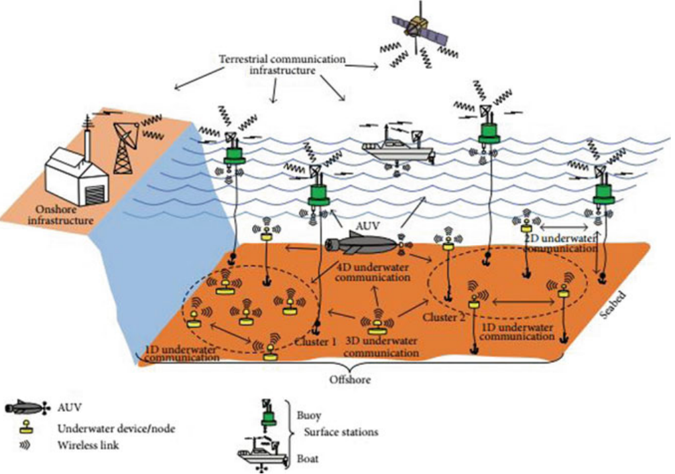
\includegraphics[width=0.7\linewidth]{images/1_underwater_sensor_networks.png}
    \caption{Underwater sensor networks architecture \cite{Nayyar}.}
    \label{fig:underwater sensor networks}
\end{figure}

In traditional marine engineering, power is transferred to underwater equipment through wet-mate subsea connectors \cite{Wang2016}. 
For the traditional methods, there have been several challenges, such as wet plug interface technology, its high cost, complex docking method, poor safety performance, and easy to be corroded by seawater. 
Fortunately, wireless power transfer (WPT) is a potential technology used to deal with these challenges because it can simplify the connection between underwater equipment and power supply, leading to reduce the continuous operating cost of underwater equipment, save a lot of resources. (, and gradually gains the favor of scholars??.)

There have been many type of energy discovered in ocean, such as tidal energy, wave energy, marine current power, ocean thermal energy, and sea salinity gradient power \cite{Capareda2019, Drew2009, Vlachogiannis2014, Zeng2020}. 
Ocean energy is rich, widely distributed, clean, and pollution-free, but low energy density and strong regionality. 
These advantages make it attractive as grid-connected energy.
(and may also make it an isolated and remote ocean energy source, thereby providing a valuable source of ocean space ({\color{red} not understand this sentence})). 
Therefore, the topic of proposing novel power solutions is attractive to researchers. 
The rapid development of applications of distributed ocean energy (such as underwater sensor networks, ocean sensors and monitoring technologies, ocean automatic network buoys, and deep-sea and tsunami buoys) is beneficial. 
One important application is to transfer power to an autonomous underwater vehicle (AUV) whose service life is recently limited by its battery power.


\section{Wireless power transfer technologies}

Broadly speaking, power is transferred without direct electrical contact between primary and secondary sides is wireless power transfer. 
Wireless power technology can be divided into two main categories, near-field (non-radiative region) wireless power transfer and far-field (radiative region) wireless power transfer. 
Near-field transmission means the distance between primary and secondary sides is within wavelength ($\lambda$) of the antenna (one of them: size of antenna or wavelength of operating frequency) \cite{}. In turn, near-field transmission is conventionally divided into two subcategories \cite{Wikipedia2021} (Distance between two antennas is denoted by $D_{range}$, and diameter of two antenna coils is denoted by $D_{ant}$.):
\begin{itemize}
    \item  Short range when the distance between two antennas is less than the diameter of antenna: $D_{range} \leq D_{ant}$. 
In this range, power is usually transferred through non-resonant capacitive or inductive coupling.
    \item Mid-range when the distance between two antennas is less than 10 times the diameter of antenna:  $D_{range} \leq 10 D_{ant}$. 
    In this range, energy is usually transferred through resonant capacitive or inductive coupling.
\end{itemize} 

\begin{table}[!t]
    \centering
    \caption{The different wireless power transmission technologies.}
    \resizebox*{\textwidth}{!}{
    \begin{tabular}{ |c|c|c|m{3.5cm}<{\centering}|m{3.5cm}<{\centering}| }
        % \thickhline
        \hline
        \textbf{Technology} & \textbf{Range} & \textbf{Frequency}         & \textbf{Antenna devices}                    & \textbf{Applications}                             \\\hline
        % \thickhline
Microwaves          & hm – km        & GHz                        & Parabolic dishes, phased arrays, rectennas  & Satellite, drone aircraft                         \\ \hline
Optical             & dam – km
                    & $\geq$THz      & Lasers, photocells, lenses & Drone aircraft, space elevator                                                                  \\ \hline
Capacitive          & cm – m         & kHz – MHz                  & Metal plate electrodes                      & Smartcards, biomedical implant
\\ \hline
Inductive           & mm – m         & Hz – GHz                   & Tuned wire coils, lumped element resonators & Electric toothbrush, smartphone, electric vehicle
\\ \hline
    \end{tabular}
    }
    \label{table:differentWPT}
\end{table}


\begin{figure}[!b]
    \resizebox*{\textwidth}{!}{
    \begin{subfigure}{0.5\textwidth}
        \centering
        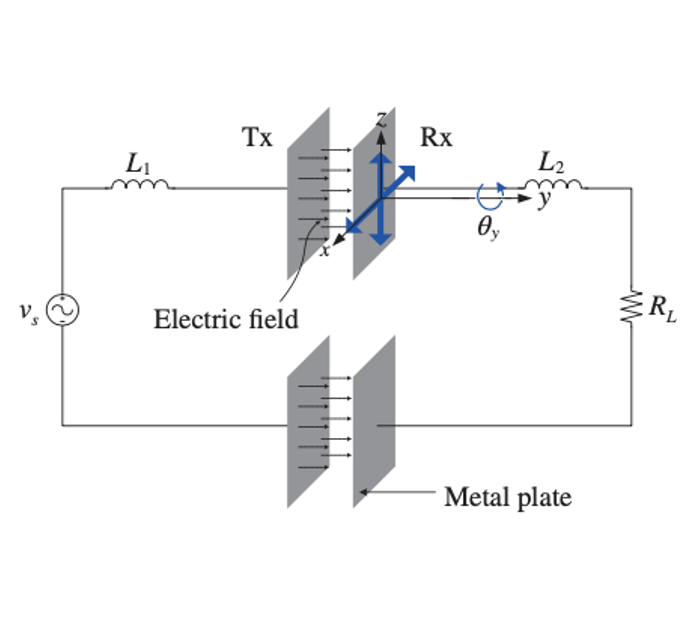
\includegraphics[width=0.9\linewidth]{images/1_capacitive_power_transfer.png}
        \caption{Capacitive power transfer \cite{Chun}.}
        \label{fig:subim1}
    \end{subfigure}
    \begin{subfigure}{0.5\textwidth}
        \centering
        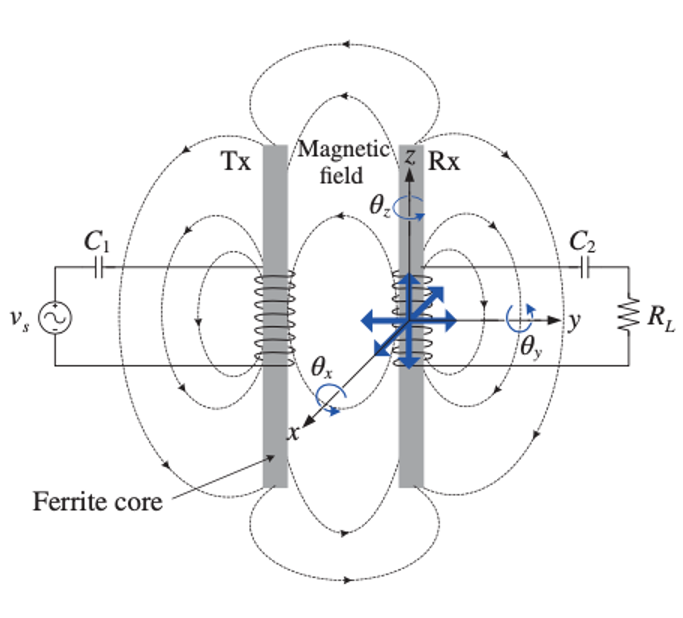
\includegraphics[width=0.9\linewidth]{images/1_inductive_power_transfer.png}
        \caption{Inductive power transfer \cite{Chun}.}
        \label{fig:subim2}
    \end{subfigure}}

    \caption{Near-field wireless power transfer.}
    \label{fig:near-fieldwpt}
\end{figure}


\begin{figure}[!t]
    \resizebox*{\textwidth}{!}{
    \begin{subfigure}{0.5\textwidth}
        \centering
        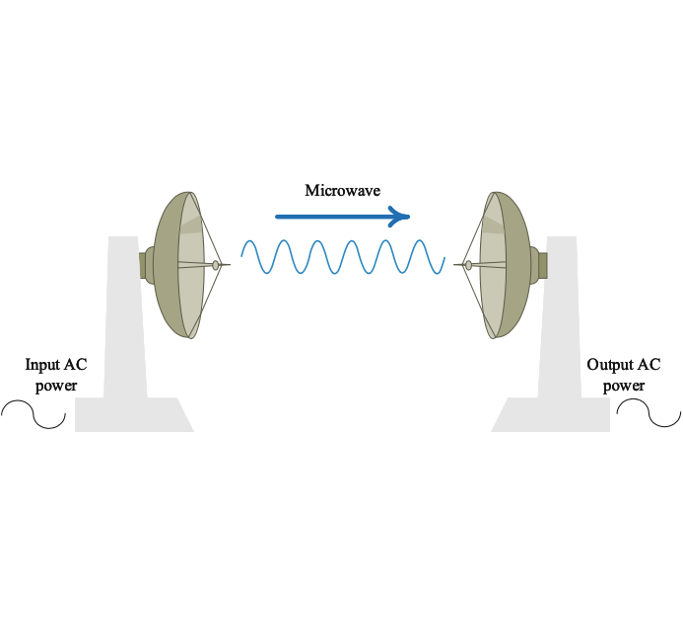
\includegraphics[width=0.9\linewidth]{images/1_microwave_power_transfer.png}
        \caption{Microwave power transfer \cite{Orekan}.}
        \label{fig:subim1}
    \end{subfigure}
    \begin{subfigure}{0.5\textwidth}
        \centering
        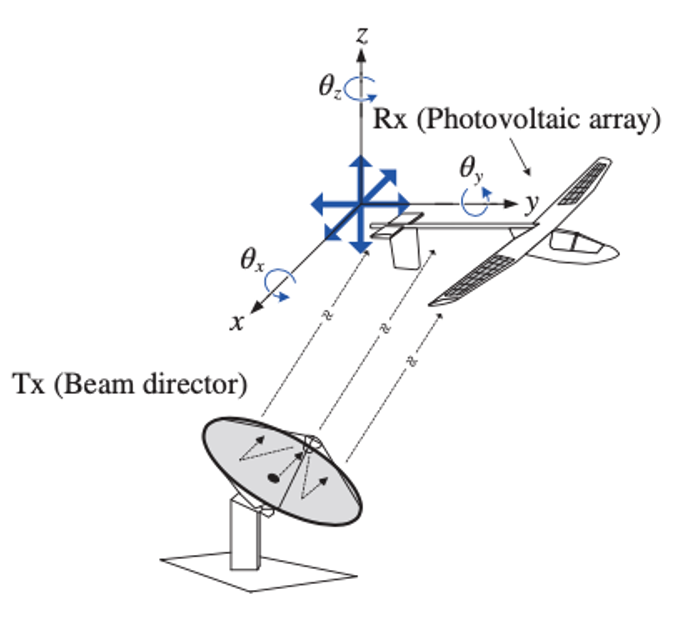
\includegraphics[width=0.9\linewidth]{images/1_laser_power_transfer.png}
        \caption{Laser power transfer \cite{Chun}.}
        \label{fig:subim2}
    \end{subfigure}
    }
    \caption{Far-field wireless power transfer.}
    \label{fig:far-fieldwpt}
\end{figure}


In contrast, in far-field WPT or radiative WPT, power is transmitted by means of electromagnetic waves, like radio waves, microwaves, or light waves. 
When the operating frequency ($f$) is relatively low, wavelength $\lambda = c/f$, at this time the diameter of the antenna is much smaller than the wavelength, $D_{ant} \ll \lambda$, and the radiated power will be very small. 
When the diameter of antenna is about wavelength, $D_{ant} \approx \lambda$, power will be radiated more efficiently. 
When the diameter of antenna is much great than wavelength, $D_{ant} \gg \lambda$, we can using high-gain antennas to concentrate electromagnetic waves on a narrow beam and directly aim at the receiver to improve transmission efficiency.


Therefore, near-field wireless power transfer systems mainly include inductive coupling power transfer and capacitive coupling power transfer (Figure \ref{fig:near-fieldwpt}). Far-field wireless power transfer systems mainly include microwave, optical, and acoustic power transfer (Figure \ref{fig:far-fieldwpt}).  The respective characteristics are shown in the table \ref{table:differentWPT}.


\section{Underwater wireless power transfer}
The applications of WPT technology has spread in many fields of science and life.
Along with the continuous development of landing application research \cite{Zhang2019}, underwater WPT technology has also attracted the researchers' attention. 
\subsection{Underwater environment}
Seawater environment has been investigated before \cite{}. It has several characteristics as follows.

\begin{itemize}
    \item Underwater and seawater environments have a blocking effect on high-frequency electromagnetic waves. 
    The distance of electromagnetic waves propagating underwater is inversely proportional to the frequency.
    Therefore, it will be difficult to achieve long-distance power transmission.
    \item Conductivity should be taken into account in theoretical analysis due to the electrical conductivity of seawater, which is often omitted in theoretical analysis of traditional wireless power transmission. 
    Recently, the system model and related theoretical analysis of underwater wireless power transfer technology has been not developed completely.
    \item The submarine landform is complex and there is undercurrent. 
    The coupler core is liable to drift under water.
    Therefore, the problem of docking between AUV and power stations becomes more challenged when transmission efficiency is sensitive to misalignment between coils.
    \item Some other impacts consist of microbial enrichment, temperature, salinity.
    
\end{itemize}

\subsection{Common UWPT systems}

\begin{figure}[!b]
    \centering
    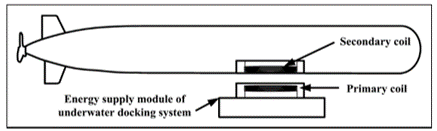
\includegraphics[width=0.7\linewidth]{images/1_stacked_UWPT_system.png}
    \caption{Stacked UWPT system \cite{Song}.}
    \label{fig:stacked UWPT system}
\end{figure}
Figure \ref{fig:stacked UWPT system} shows a stacked UWPT system, this study was completed by Baowei Song et al \cite{Song}. They achieved a transmission efficiency of 72\% while maintaining 100w output power.
They are using a saddle structure transmitter (Details as shown in figure \ref{fig:stacked UWPT system detail}) and a deformed cylindrical receiver. This structure is very convenient for AUT to park, but because there is no stable protection structure, it is also easy to shift when charging.

\begin{figure}[!b]
    \centering
    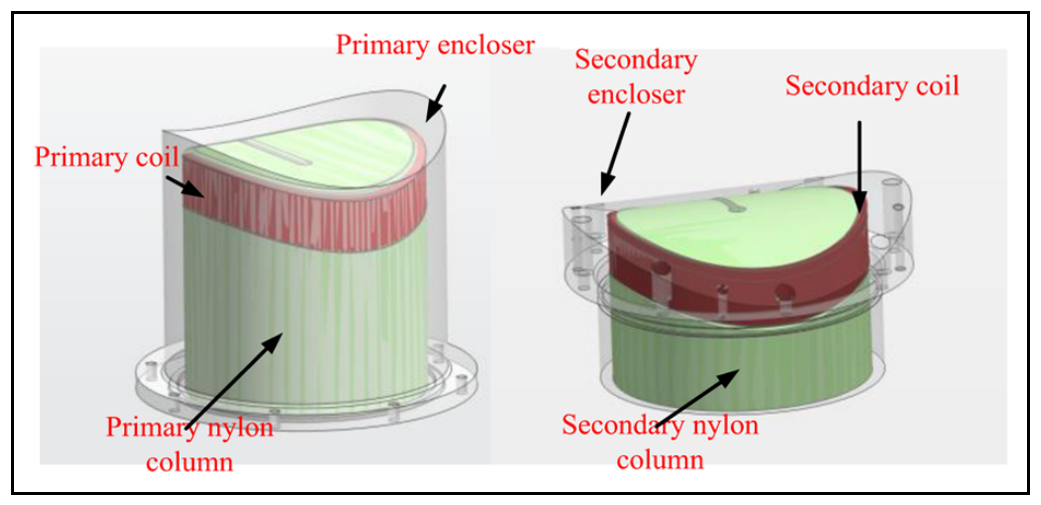
\includegraphics[width=0.7\linewidth]{images/1_stacked_UWPT_system_details.png}
    \caption{The primary and secondary coils of stacked UWPT system \cite{Song}.}
    \label{fig:stacked UWPT system detail}
\end{figure}

Figure \ref{fig:plug in UWPT system} shows the plug-in UPWT system. 
It is clear that the AUV needs to be moved into a hollow cylindrical structure transmitter.
Conventionally, it will be difficult to park accurately. 
However, this structure can maintain the stability of the AUV during AUV charging so that the system charging is more secure. 
Another advantage of this structure is that the receiving coil is relatively large, which can bring out high mutual inductance. 
As a result, this system can transmit high power to receiver.
However, ({\color{red} you have to mention the disadvantage of this system (magnetic flux at center of AUV is very strong, it affect the operation inside UAV, ...). It will be your motivation to do this research})
Therefore, in order to address this issue, we propose coil-array structure UWPT system.
\begin{figure}[!t]
    \centering
    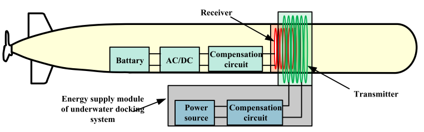
\includegraphics[width=0.7\linewidth]{images/1_plugin_UWPT_system.png}
    % \caption{Plug-in UWPT system [wang].}
    \caption{Plug-in UWPT system \cite{Wang2019}.}
    \label{fig:plug in UWPT system}
\end{figure}


\section{The main research content of this thesis}
This thesis mainly investigates the difference between IPT systems in underwater environment and in air environment. 
Then, considering the durability and high reliability of underwater AUV, we proposes a novel coil-array power transfer system. 
This research can be considered as a reference material for subsequent researches on the IPT system using multiple coil in underwater environment.

\section{Roadmap}
Chapter ?? describes the background of this research as well as the purpose and the significance of the research.
The characteristics and advantages and disadvantages of mainstream WPT technology are analyzed to give a general look at IPT systems used for transmitting power in underwater environment. 
(A detailed summary and analysis of the current research status of related technologies at home and abroad, including underwater wired energy transmission technology, WPT technology in underwater and air media, and an explanation of the research focus of this article $\rightarrow$ do not understand).

Chapter ?? focuses on the basic theory of inductive power transmission. 
First, the basic IPT model is mentioned and its principle is analyzed. 
Then, popular technology of compensation network is presented to show how compensation network affect load voltage. Finally, the underwater IPT system model is illustrated.

Chapter ?? initially explores the influence of the underwater environment on IPT systems. 
First, by measuring the Z-paremeter of the IPT system in three different media to observe the changes . 
Then Z-parameter is investigated against the changes of the size of the internal coil. 
Finally, Z-parameter of the IPT system is evaluated when changing different working frequencies.

Chapter ?? first studies the magnetic field characteristics of the different coil structures.
It focuses on the analysis of the coil size and distance effect on the coil magnetic field.
Then, we simulates the magnetic field distribution of the coil containing the air gap core.
After that, we proposes a new type of coil-array structure. 
The simulations is carried out by WIPL-D software to illustrate the comparison of the magnetic field distribution and transmission efficiency between the coil-array coil structure and the two-ring structure. 
Then through experiments, we evaluate the performance of the IPT systems under several different coil-array arrangements. Summarize the advantages and disadvantges of different arrangements.

Chapter five summarizes the thesis. 
In response to these shortcomings, some suggestions to improve the performance of the IPT systems are put forward in the future work.








